\documentclass[12pt,a4paper]{article}
\usepackage[utf8]{inputenc}
\usepackage{amsmath}
\usepackage{listings}
\usepackage{verbatim}
\usepackage{graphicx} 
\oddsidemargin 0cm
\marginparwidth 0cm
\hoffset 0cm
\usepackage{polski}
\begin{document} 
\large
\begin{tabular}{|c|c|c|c|}
\hline
\multicolumn{4}{|l|}{Temat:}\\
\multicolumn{4}{|c|}{Rozwiązywanie UARL metodami bezpośrednimi (1)}\\
\hline
\multicolumn{1}{|l}{Wykonał:}&\multicolumn{1}{|l}{Wydział:}&\multicolumn{1}{|c}{Kierunek}&\multicolumn{1}{|l|}{Grupa:}\\
Marcin Fabrykowski&FiIS&Inf. Stos.&grupa 3\\
\hline
\end{tabular}
\normalsize
\vspace{2cm}
\begin{enumerate}
\item Metoda eliminacji Gaussa-Jordana\\
Metoda ta pozwala na redukcje zadanej macierzy do macierzy jednostkowej.\\
Mając układ równań np:
\begin{align}
2*x_0+4*x_1+6*x_2&=46\\
\nonumber 7*x_0+1*x_1+2*x_2&=34\\
\nonumber 4*x_0+4*x_1+4*x_2&=40
\end{align}
Zamieniamy miejscami wiersz 1 i 2:
\begin{align}
7*x_0+1*x_1+2*x_2&=34\\
\nonumber 2*x_0+4*x_1+6*x_2&=46\\
\nonumber 4*x_0+4*x_1+4*x_2&=40
\end{align}
Dzielimy wiersz pierwszy przez $a_{11}=7$
\begin{align}
1*x_0+0.143*x_1+0.286*x_2&=4.857\\
\nonumber 2*x_0+4*x_1+6*x_2&=46\\
\nonumber 4*x_0+4*x_1+4*x_2&=40
\end{align}
Następnie odejmujemy od pozostałych wierszy wiersz pierwszy pomnożony przez odpowiedni współczynnik $a_{i1}$,\\Dla wiersza 2: $a_{21}=2$
\begin{align}
1*x_0+0.143*x_1+0.286*x_2&=4.857\\
\nonumber 0*x_0+3.714*x_1+5.429*x_2&=36.286\\
\nonumber 0*x_0+3.429x_1+2.857*x_2&=20.571
\end{align}
Następnie dzielimy wiersz drugi przez współczynnik $a_{22}=3.714$
\begin{align}
1*x_0+0.143*x_1+0.286*x_2&=4.857\\
\nonumber 0*x_0+1*x_1+1.462*x_2&=9.769\\
\nonumber 0*x_0+3.429x_1+2.857*x_2&=20.571
\end{align}
I podobnie jak wcześniej, odejmujemy go od pozostałych wierszy, mnożąc przez $a_{i2}$
\begin{align}
1*x_0+0*x_1+0.077*x_2&=3.460\\
\nonumber 0*x_0+1*x_1+1.462*x_2&=9.769\\
\nonumber 0*x_0+0*x_1-2.154*x_2&=-12.923
\end{align}
Analogicznie postępujemy z wierszem 3:
\begin{align}
1*x_0+0*x_1+0.077*x_2&=3.460\\
\nonumber 0*x_0+1*x_1+0*x_2&=0.997\\
\nonumber 0*x_0+0*x_1+1*x_2&=6
\end{align}
Odejmujemy:
\begin{align}
1*x_0+0*x_1+0*x_2&=2.998\\
\nonumber 0*x_0+1*x_1+0*x_2&=0.997\\
\nonumber 0*x_0+0*x_1+1*x_2&=6
\end{align}
Z powyższego układu równań wynika wprost, że:
\begin{align}
x_0&=2.998\\
\nonumber x_1&=0.997\\
\nonumber x_2&=6
\end{align}
\item Wykonanie ćwiczenia\\
Celem ćwiczenia jest rozwiązanie zadanej macierzy:\\
\footnotesize
\begin{equation}
\begin{pmatrix}
1&0&0&0&0&0&0\\
-1&1&0&0&0&0&0\\
1&(\omega^2h^2-2)&1&0&0&0&0\\
0&1&(\omega^2h^2-2)&1&0&0&0\\
0&0&1&(\omega^2h^2-2)&1&0&0\\
0&0&0&1&(\omega^2h^2-2)&1&0\\
0&0&0&0&1&(\omega^2h^2-2)&1
\end{pmatrix}
\begin{pmatrix}
x_0\\
x_1\\
x_2\\
x_3\\
x_4\\
x_5\\
x_6
\end{pmatrix}
=
\begin{pmatrix}
A\\
\upsilon_0h\\
0\\
0\\
0\\
0\\
0
\end{pmatrix}
\end{equation}
Do tego celu uzyjemy własnoręcznie napisanego programu, wykorzustującego biblioteki numeryczne \textit{nrutil}
\lstinputlisting[language=C++,caption=main.cpp]{main.cpp}
W efekcie czego otrzymamy wynik:
\small
\lstinputlisting[basicstyle=\footnotesize,caption=dane.dat]{dane.dat}
\normalsize
Co po wygenerowaniu wykresu przy użyciu programu Gnuplot skryptem:
\lstinputlisting[language=Gnuplot,caption=plot.sh]{plot.sh}
da nam wynik jak na Rys. \ref{fig:wynik}
\begin{figure}
\caption{Wynik}
\label{fig:wynik}
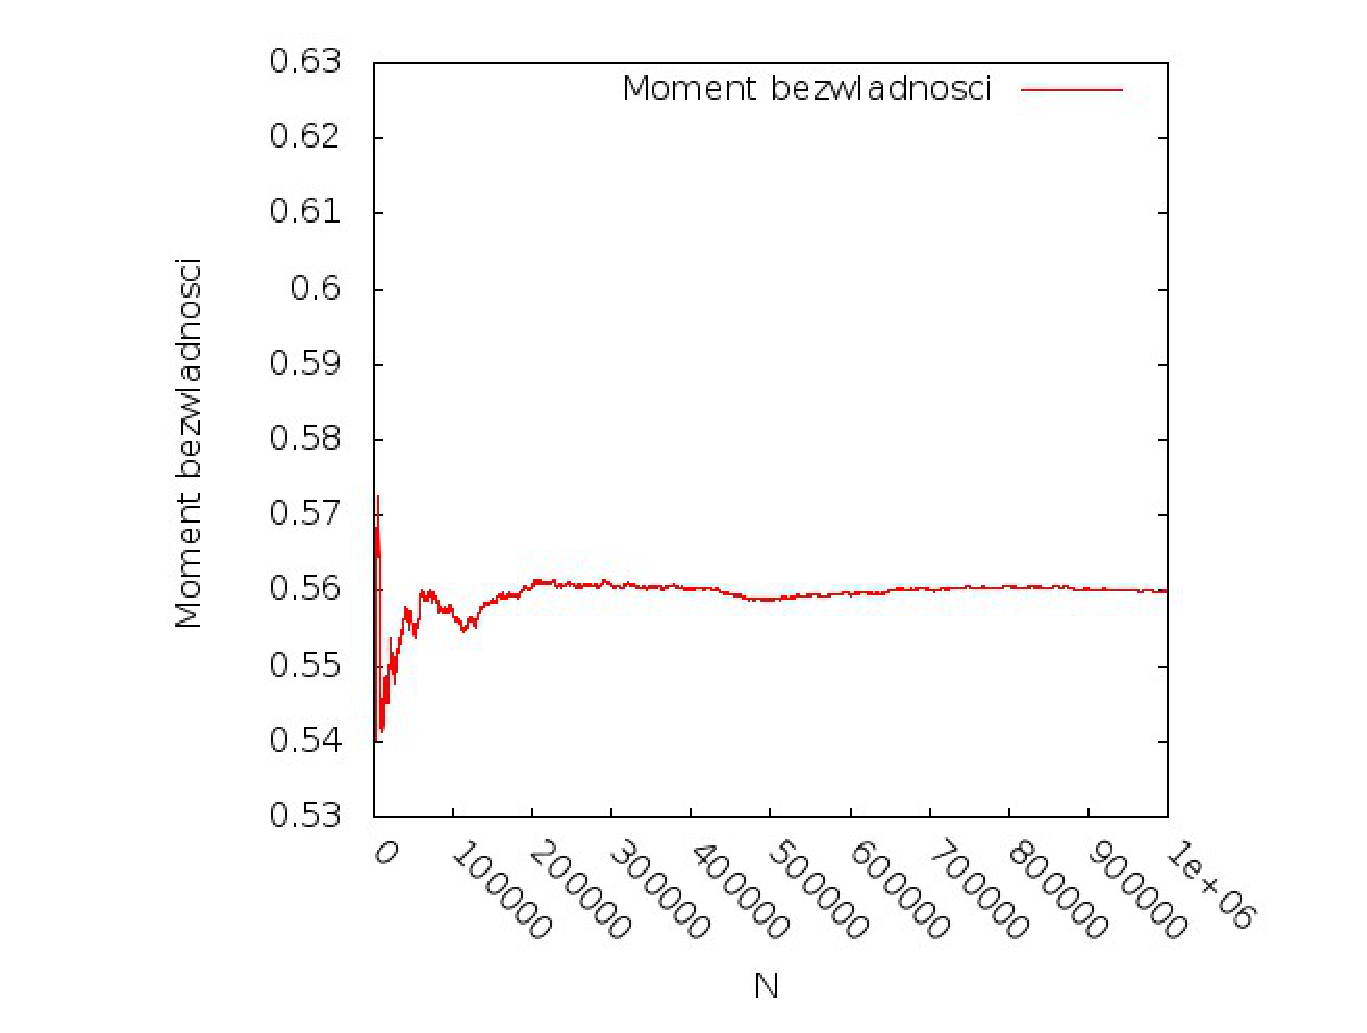
\includegraphics{plot.eps}
\end{figure}
\item Wniski\\
Jak widać na wykresie, wynik jest zgodny z przewidywanym, co może świadczyć o poprawności metody. Trzeba jednak zwrócić uwagę na ewentualne niedokładności wynikające z dokładności zapisu liczb zmiennoprzecinkowych.\\
Ponadto, metoda Gaussa-Jordana sprawdza się przy małych macierzach. w przypadku większych macierzy algorytm jest nieefektywny:\\
dla h=0.1:
\begin{verbatim}
i9fabryk@fatcat:~/numerki/1$ time ./main 
n=179

real    0m0.094s
user    0m0.080s
sys     0m0.000s
\end{verbatim}
natomiast dla h=0.01:
\begin{verbatim}
i9fabryk@fatcat:~/numerki/1$ time ./main 
n=1800

real    1m22.110s
user    1m21.770s
sys     0m0.130s
\end{verbatim}
\begin{verbatim}
i9fabryk@fatcat:~/numerki/1$ time ./main 
n=17999
^C

real    3m40.085s
user    3m38.290s
sys     0m1.640s
\end{verbatim}
Program nie zakończł działania w rozsądnym czasie. Przypuszczalny oczekiwany czas to 24h.

\begin{tabular}{|c|c|}
\hline
h&czas [s]\\
\hline
0.1&0.094\\
0.01&88.110\\
0.001&???\\
\hline
\end{tabular}
\end{enumerate}
\end{document}
